\documentclass[english]{presentation}
%\setbeameroption{show notes on second screen}
%\setbeameroption{show only notes}

\usepackage{chngpage}
\usepackage{array}

% Presento style file
\usepackage{config/presento}

\usepackage{textpos}
\setlength{\TPHorizModule}{1cm}
\setlength{\TPVertModule}{1cm}

\usepackage{stmaryrd}

% strikethrough text
\usepackage[normalem]{ulem}

% macros
\usepackage{mama}

\renewcommand{\O}{\mathcal{O}}

\renewcommand<>{\sout}[1]{%
	\alt#2{\beameroriginal{\sout}{#1}}{#1}%
}

\AtBeginDocument{%
 \abovedisplayskip=1ex
 \belowdisplayskip=1ex
 \abovedisplayshortskip=0pt
 \belowdisplayshortskip=7pt minus 4pt
}

\title{Fantastic sheaves\\[.8ex]and where to find them}
\subtitle{An MSP101 talk}
\institute{University of Strathclyde}
\author{Matteo Capucci}
\date{October 22, 2020 (Day 300 of the COVID Era)}

\begin{document}
	\begin{frame}[plain]
		\maketitle
	\end{frame}

	\begin{frame}{Overview}
	\textbf{Goal}: to show sheaves are useful modelling gadgets.

	\vspace{5ex}

	Two avenues:
	\begin{enumerate}
		\item \textbf{Geometry}: local-to-global behaviour, cohomology
		\item \textbf{Logic}: local modalities, system specifications, models
	\end{enumerate}
\end{frame}

	\begin{frame}{Basics}
	Let $X$ be a topological space, $\O(X)$ its frame of open sets.

	\begin{definition}
		A \defining{presheaf} on $X$ is a functor
		\begin{equation*}
			F: \O(X)^\op \longto \Set
		\end{equation*}
		%(A presheaf of $\cat C$s is a functor $\O(X)^\op \to \cat C$)
	\end{definition}

	Elements of $F(U)$ are called \defining{sections}. The map $F(V \subseteq U)$ is called \defining{restriction}, and we write $s\vert_V := F(V \subseteq U)(s)$.

	\begin{definition}
		A \defining{sheaf} on $X$ is a presheaf $F$ such that for every open covering $\{U_i\}_{i \in I}$:
		\begin{equation*}
			\textbf{sheaf condition}: \quad F(\colim U_i) \iso \lim F(U_i).
		\end{equation*}
	\end{definition}
	The sheaf condition is a `continuity' or a `locality' condition.
\end{frame}

\begin{frame}{Sheaf condition}
	Let's unpack it:
	\vfill
	\begin{enumerate}
		\item The colimit of a covering is
		\begin{equation*}
			{\textstyle \colim U_i = \bigcup_i U_i =: U}.
		\end{equation*}
		Elements of $F(U)$ are `globally defined sections' (wrt to $U$).
		\vspace{3ex}
		\item Elements of $\lim F(U_i)$ are `locally defined sections' which satisfy a \defining{compatibility condition}:
		\begin{equation*}
			\lim F(U_i) = \{(s_i)_{i \in I} \suchthat s_i \vert_{U_i \cap U_j} = s_j \vert_{U_i \cap U_j}\ \text{for all $i,j \in I$}\}
		\end{equation*}
		\vspace{1ex}
		\item There is a universal morphism
		\begin{eqalign*}
			\varphi : F(\colim U_i) &\longto \lim F(U_i)\\
			s &\longmapsto (s\vert_{U_i})_{i \in I}
		\end{eqalign*}
	\end{enumerate}
	\vfill
\end{frame}

\begin{frame}{Sheaf condition}
	\begin{eqalign*}
		\varphi : F(\colim U_i) &\longto \lim F(U_i)\\
		s &\longmapsto (s\vert_{U_i})_{i \in I}
	\end{eqalign*}
	Then:
	\begin{enumerate}
		\item $\varphi$ mono means
		\begin{center}
			\textbf{separation axiom}:\quad $s=t \in F(U)$ iff $s\vert_{U_i} = t\vert_{U_i}$ forall $i \in I$.
		\end{center}
		\item $\varphi$ epi means
		\begin{center}
			\textbf{glueing axiom}:\quad every compatible assignment of sections $(s_i)_{i \in I} \in \lim F(U_i)$ `glues' to a global section $s \in F(U)$.
		\end{center}
	\end{enumerate}
	\vfill
	A presheaf satisfying separation is called \defining{separated}.

	A sheaf satisfies both.
\end{frame}

\begin{frame}{Sheaf condition}
	\begin{example}
		The canonical example is $C(-; \R)$ of continuous real functions.\\
		Also: smooth functions, measurable functions, etc. (in fact many structures can be encoded directly in a \emph{structure sheaf}).
	\end{example}
	\begin{block}{Non-example}
		Separated presheaves which are not sheaves:
		\begin{enumerate}
			\item Constant functions: if $U$ and $V$ are disjoint open sets, there's no way to glue two constant functions with different values on $U$ and $V$, \emph{even though they agree on $U \cap V$}.
			\item Bounded functions: choose an infinite covering, even though every local section might be bounded there's no guarantee their glueing will be bounded (e.g. $\lambda x.x^2\vert_{(n,n+1)}$)
		\end{enumerate}
	\end{block}
	\setnote{Non-separated presheaves are rare to find in practice (though easy to construct)}
\end{frame}

% \begin{frame}{Sheaf condition}
% 	In general: `local properties' (continuity, smoothness) work, `global' not so much (constancy, boundedness).
% 	\begin{example}
% 		If we ask for the `local versions', constant and bounded presheaves become sheaves:
% 		\begin{enumerate}
% 			\item Constant sheaf at $A$: $\underline A(U)$ = locally constant maps $U \to A$. Then we can glue without problems.
% 			\item The sheaf of locally bounded functions.
% 			\item Integrability is also a non-local property, hence $L^1$ is not a sheaf but a presheaf, unless we ask for \emph{local} integrability ($L^1_{\text{loc}}$).
% 		\end{enumerate}
% 	\end{example}
% \end{frame}

\begin{frame}{Sheaf condition}
	The sheaf condition can be read also in terms of \textbf{systems theory}:
	\vfill
	Suppose $X$ is a `system', and its open sets are `parts'.%\setnote{(later we'll describe a formalism which allows to relax the assumption `parts form a topology' [which isn't that bad anyway])}

	Then the \textbf{functor of behaviours} is a presheaf:
	\vfill
	\begin{diagram*}
		U \&[-3ex] \&[-1ex] \{\text{behaviours of the part $U$}\} \arrow{dd}{\text{behaviour induced by forgetting $U \setminus V$}}\\[-6ex]
		\phantom{A} \& \arrow[mapsto]{r}{B} \& \phantom{AAAAAAAAAAAaaAAAAAAAA} \\[-6ex]
		V \arrow{uu}{\subseteq} \&\& \{\text{behaviours of the part $V$}\}
	\end{diagram*}
	\vfill
	\onslide<2->{
		\begin{description}
			\item[Separation:] \emph{behaviours can be distinguished at the level of parts}. %{\onslide<2>{\color{coloraccent}Fails if we have emergent effects!}}
			\item[Glueing:] \emph{compatible behaviours of the parts form global behaviours}. %\onslide<2>{\color{coloraccent}{Always ok.}}
		\end{description}
	}
\end{frame}

\begin{frame}{Sheafification}
	The inclusion of sheaves into presheaves has a left adjoint:
	\begin{diagram*}
		\Sh(X) \arrow[hook, shift right, swap]{r}{i} \& \Psh(X) \arrow[shift right, swap]{l}{\cdot^a}
	\end{diagram*}
	Informally, you get it by putting `locally' in front of properties.
	\onslide<2->\begin{example}
		\begin{enumerate}
			\item %$(\text{constant maps at $A$})^a =$ constant \emph{sheaf} at $A$:
			%\begin{center}
				$\underline S^a(U)$ = {\color{red}locally} constant maps $U \to S$ \setnote{(constant \emph{sheaf} at $S$)}
			%\end{center}
			\item
			%\begin{center}
				$Bdd^a_\R(U)$ = {\color{red}locally} bounded maps $U \to \R$
			%\end{center}
		\end{enumerate}
	\end{example}
	In general,
	\begin{center}
		$F^a(U) = {\displaystyle \colim_{\mathcal{U}\ \text{hyper.}} \lim F(\mathcal{U})}$ = formal glueings over (hyper)covers
	\end{center}
\end{frame}

	\begin{frame}{$\Underset{\only<2->{\color{red}\check{C}ech}}{\text{\sout<2->{Sheaf}}}$ cohomology}
	Hence:
	\begin{center}
	\bfseries
		(pre)sheaves mediate the passage from local to global.
	\end{center}

	Most importantly, they enable the right tooling to study obstructions to this passage, namely \textbf{$\Underset{\only<2->{\color{red}\check{C}ech}}{\text{\sout<2->{sheaf}}}$ cohomology}.

	\vfill

	\onslide<3->{
		Reasons to prefer \v{C}ech to plain cohomology:
		\begin{enumerate}
			\item It's computational \setnote{(it's a simplicial cohomology in disguise)}
			\item Easily generalized to non-abelian sheaves (e.g. $\Set$-sheaves)\\
		\end{enumerate}
		For this talk though, let's stick to the \emph{abelian} version, hence we will assume \emph{$F$ is a sheaf valued in $\Ab$} \setnote{(or any abelian cat if you know what that means)}
	}
\end{frame}

\begin{frame}{\v{C}ech cohomology}
	Take a `good' cover $\{U_i\}_{i \in I}$ of $X$. \setnote{(e.g. contractible intersections)}
	\vfill
	Consider the following \textbf{cochain complex}: \setnote{(meaning $\im d_n \subseteq \ker d_{n+1}$)}
	\vspace{4ex}
	\begin{diagram*}
		0 \arrow{r} \&[-6ex] \prod_i F(U_i) \arrow{r}{d_0} \&[-5ex] \prod_{i,j} F(U_i \cap U_j) \arrow{r}{d_1} \&[-5ex] \prod_{i,j,k} F(U_i \cap U_j \cap U_k) \arrow{r}{d_2} \&[-5ex] \cdots
	\end{diagram*}
	\vfill
	whose \defining{coboundaries} are
	\vspace{4ex}
	\begin{eqalign*}
		d_0((s_i)_i) &= (s_i \vert_{U_i \cap U_j} - s_j \vert_{U_i \cap U_j})_{i,j}\\
		d_1((s_{i,j})_{i,j}) &= (s_{i,j}\vert_{U_i \cap U_j \cap U_k} - s_{j,k}\vert_{U_i \cap U_j \cap U_k} + s_{k,i}\vert_{U_i \cap U_j \cap U_k})_{i,j,k}\\
		&\ \ \vdots
	\end{eqalign*}
	\vfill
\end{frame}

\begin{frame}{\v{C}ech cohomology}
	The cohomology of the complex measures how far is $\im d_n$ from coinciding with $\ker d_{n+1}$: \setnote{('exactness')}
	\begin{diagram*}
		0 \arrow{r} \&[-6ex] \prod_i F(U_i) \arrow[squiggly, colornote]{d} \arrow{r}{d_0} \&[-5ex] \prod_{i,j} F(U_i \cap U_j) \arrow[squiggly, colornote]{d} \arrow{r}{d_1} \&[-5ex] \prod_{i,j,k} F(U_i \cap U_j \cap U_k) \arrow[squiggly, colornote]{d} \arrow{r}{d_2} \&[-5ex] \cdots\\[-5ex]
		\& H^0 = \ker d_0 \& H^1 = \dfrac{\ker d_1}{\im d_0} \& H^2 = \dfrac{\ker d_2}{\im d_1}
	\end{diagram*}
	\onslide<2->{
		Meaning:
		\begin{eqalign*}
			H^0 &= \text{local sections $(s_i)_i$ s.t. $s_i\vert_{U_i \cap U_j} = s_j\vert_{U_i \cap U_j}$ $\forall i,j \in I$}\\
			&\overset{\text{if sheaf}}= \text{\color{red}global sections}.\\
			H^1 &= \text{compatible local sections on $U_i \cap U_j$}\\
			&\phantom{=}\ \ \text{which do not arise from an assignment on the opens}\\
			&\approx \text{\color{red}$1$-holes}\\
			H^n &= \cdots \approx \text{\color{red}$n$-holes}
		\end{eqalign*}
	}
\end{frame}

\begin{frame}{\v{C}ech cohomology: example}
	\vspace{1ex}
	\begin{minipage}[b]{\textwidth}
		\begin{minipage}{.4\textwidth}
			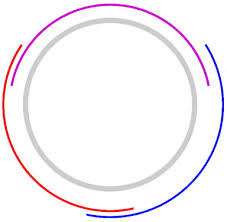
\includegraphics[width=.6\columnwidth]{figures/s1_cover.png}
		\end{minipage}%
		\begin{minipage}{.6\textwidth}
			Cover $S^1$ as in the picture,\\let $F = \Delta K = $ constant sheaf at $K$ field.
			\begin{diagram*}
				\text{\v{C}ech complex:} \quad 0 \arrow{r} \&[-5ex] K^3 \arrow{r}{d_0} \&[-5ex] K^3 \arrow{r}{d_1} \&[-5ex] 0
			\end{diagram*}
		\end{minipage}
	\end{minipage}
	\vspace{1ex}
	\onslide<2->{
		\begin{eqalign*}
			d_0 &= \begin{pmatrix}
				1 & -1 & 0\\
				0 & 1 & -1\\
				-1 & 0 & 1
			\end{pmatrix}\onslide<3->{\implies \operatorname{rk}(d_0) = 2 \implies \!\begin{cases}
				\dim \ker d_0 = 1,\\
				\dim \im d_0 = 2
			\end{cases}}\\[2ex]
			\onslide<4->{d_1 &= 0} \phantom{xxxxxxxxxxxxxxxxxxxxxxxxxxxxxx}\; \onslide<5->{\implies \dim \ker d_1= 3}\\
		\end{eqalign*}
	}
	\onslide<6->{
		Hence
		\vspace{-3ex}
		\begin{center}
			\begin{minipage}{.4\textwidth}
				\begin{eqalign*}
					H^{\color{blue}0} &= K^{\color{red}1}\\
					H^{\color{blue}1} &\iso K^3/K^2 \iso K^{\color{red} 1}\\
					H^{\color{blue}n} &= 0 \iso K^{\color{red}0}
				\end{eqalign*}%
			\end{minipage}%
			\begin{minipage}{.45\textwidth}%
				\begin{eqalign*}
					&\text{{\color{red}1} {\color{blue}0}-hole = 1 connected component}\\
					&\text{{\color{red}1} {\color{blue}1}-hole}\\
					&\text{{\color{red}0} {\color{blue}n}-holes for all $n \geq 2$}
				\end{eqalign*}
			\end{minipage}
		\end{center}
	}
\end{frame}

\begin{frame}{\v{C}ech cohomology}
	Cohomology is not completely determined by the topology of the space though, it is really determined by the structure of the sheaf \setnote{(it's the cohomology of its étalé space)}.
	\vfill
	\begin{example}
		\vspace{1.5ex}
		\begin{minipage}{.2\textwidth}
			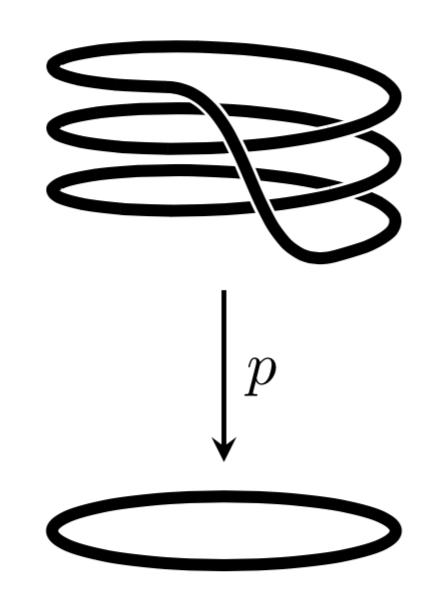
\includegraphics[width=.8\columnwidth]{figures/s1_triple_covering.png}
		\end{minipage}
		\begin{minipage}{.7\textwidth}
			Repeat the previous computation with a different \emph{locally} constant sheaf.
		\end{minipage}
	\end{example}
	\vfill
	Hence \textbf{topological obstructions $\neq$ local-to-global obstructions}!
\end{frame}

\begin{frame}{\v{C}ech cohomology: systems theory}
	% In terms of systems theory, \textbf{cohomology detects generative effects}.
	% \vfill
	Let $B$ {\color{colornote}(presheaf of behaviours)} be a \textbf{pre}sheaf of abelian groups, let $\{U_i\}_{i \in I}$ be an open covering of $U$.

	Its \textbf{{\color{red}{augmented}} \v{C}ech complex} is:
	\begin{diagram*}
		0 \arrow{r} \&[-5ex] \color{red}{B(U)} \arrow[visible on=<2->, squiggly, colornote]{d} \arrow[red]{r}{d_{-1}} \&[-5ex] \prod_i B(U_i) \arrow[visible on=<2->, squiggly, colornote]{d} \arrow{r}{d_0} \&[-5ex] \prod_{i,j} B(U_i \cap U_j) \arrow[visible on=<2->, squiggly, colornote]{d} \arrow{r}{d_1} \&[-5ex] \cdots\\[-5ex]
		\&[-5ex] \onslide*<2->{\color{blue}{H^{-1} = \ker d_{-1}}} \& \onslide*<2->{\color{blue}{H^0 = \dfrac{\ker d_0}{\im d_{-1}}}} \& \onslide*<2->{H^1 = \dfrac{\ker d_1}{\im d_0}} \& \onslide*<2->{\cdots}
	\end{diagram*}
	where {\color{red}$d_{-1}(s) = (s\vert_{U_i})_i$}.
	\begin{eqalign*}
		\onslide<3->{H^{-1} &= \text{failure of $B$ to be separated \color{colornote}{($=0$ iff separation holds)}}}\\
		&\qquad\onslide<6->{\rightsquigarrow \text{\color{red}\textbf{extensionality of behaviour} ($=0$ if fully extensional)}}\\
		\onslide<4->{H^0 &= \text{failure of $B$ to glue \color{colornote}{($=0$ iff glueing holds)}}}\\
		&\qquad\onslide<7->{\rightsquigarrow \text{{\color{red}\textbf{emergent behaviour} ($=0$ if no emergence)} \cite{adam2017systems}}}\\
		\onslide<5->{H^{\geq 1} &= \text{same as before!}}\onslide<8->{\rightsquigarrow \text{\color{red}\textbf{higher-order emergent behaviour...?}}}\\
	\end{eqalign*}
\end{frame}

	% \begin{frame}{Logic}
% 	\begin{center}
% 		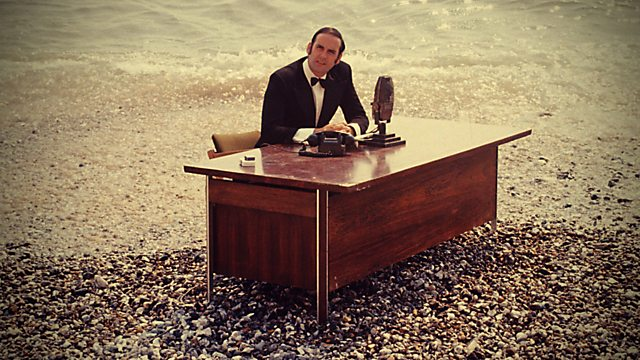
\includegraphics[width=\textwidth]{figures/something_different.jpg}
% 	\end{center}
% 	%We would like to define \textbf{sheaves on arbitrary categories}: in fact, there are presheaves on any category, why shouldn't we have sheaves?
% \end{frame}

\begin{framecard}
	{\color{white}
	\bfseries

	\hugetext{Logic}}
\end{framecard}

\begin{frame}{Logic}
	\textbf{Idea}:
	\begin{center}
		\color{red}
		\bfseries
			sheaves are 'locally defined sets' on a 'site'.
	\end{center}

	\vspace{5ex}

	We are going to see
	\begin{enumerate}
		\item Sites \& topoi
		\item The internal language of a topos of sheaves
		\item The `locally' modality
		\item Logical-flavoured applications: forcing, internalization
	\end{enumerate}
\end{frame}

\begin{frame}{Sites}
	Let $\cat C$ be a small category.
	\begin{definition}
		A \defining{sieve} on $U \tin \cat C$ is a collection $S$ of morphisms $\{U_i \to U\}_{i \in I}$ closed by precomposition on the left:
		\begin{equation*}
			\underbrace{V \to \underbrace{U_i \to U}_{\in S}}_{\implies \in S}
		\end{equation*}
		\setnote{You generate a sieve by choosing some morphisms into $U$ and then closing.}
	\end{definition}

	\begin{definition}<2->
		A \defining{site} is a small category $\cat C$ together with a \defining{Grothendieck topology} $J$, i.e. a choice of sieves for each object $U \tin \cat C$:
		\begin{equation*}
			J(U) = \text{\bfseries covering sieves for $U$}
		\end{equation*}
		\setnote{such that $J(U)$ satisfies some very reasonable conditions.}
	\end{definition}
\end{frame}

\begin{frame}{Sites}
	\begin{definition}
		Let $(\cat C, J)$ be a site.
		A presheaf $F : \cat C^\op \to \Set$ is a sheaf iff for every $U \tin \cat C$ and any \emph{covering sieve} $S \in J(U)$,
		\begin{equation*}
			F(U) \iso \lim F(S).
		\end{equation*}
		\textbf{Warning}: it's not always true that $U \iso \colim S$!
	\end{definition}

	\begin{example}<2->
		For $X$ topological space:
		\begin{eqalign*}
			\Sh X  &= \Sh (\O(X),\, \text{open coverings})\\
			\Psh X &= \Sh (\O(X),\, \text{trivial coverings})
		\end{eqalign*}
	\end{example}
	\onslide<3->{
		\textbf{Takeaway}: locality is not a fixed concept! It depends on the topology, but not the one you expect.
	}
\end{frame}

\begin{frame}{The topos of presheaves}
	Let $X$ be a site. $\Sh X$ inherits a lot of structure from $\Set$:
	\begin{enumerate}
		\item {[Finite]} \textbf{completeness} and \textbf{cocompleteness} (pointwise co/limits)
		\item \textbf{Exponentials}:
		\begin{equation*}
			G^F(U) \iso \Nat(\yo U, G^F) \iso \Nat(\yo U \times F, G)
		\end{equation*}
		\item \textbf{Subobject classifier}: $\Omega(U) =$ `principal covering sieves on $U$'.
		\begin{diagram*}
			P \arrow[tail, swap]{d}{\forall \varphi} \arrow{r}{!} \& 1 \arrow{d}{\true} \&[-3ex] \color{colornote}{*} \arrow[colornote, mapsto]{d}\\
			F \arrow{r}{\exists ! \ulcorner \varphi \urcorner} \& \Omega \& \color{colornote}{1_U}
		\end{diagram*}
		\begin{diagram*}
			\phantom{XXX} \color{colornote}{s \in F(U)} \arrow[colornote, mapsto]{r} \& \color{colornote}{\{ V \nto{f} U \suchthat s\vert_f \in P(V) \}}
		\end{diagram*}%
		Intuition: `ways $s$ enters in $P$ at $U$'.\\
		$P(s)$ true at $U$ \underline{iff} $s$ entered through $1_U$ \underline{iff} $s \in P(U)$ already.
	\end{enumerate}
\end{frame}

\begin{frame}{Internal language of topoi}
	A category satisfying these properties is called an \defining{elementary topos}.\\
	A topos $\simeq$ to a topos of sheaves on a site is called \defining{Grothendieck}.

	\vfill

	The definition is tailored to provide a rich \textbf{internal language}:

	\begin{center}
		\begin{tabularx}{\textwidth}{XX}
			$A$ type & $A$ object\\[1.5ex]
			$t(x) \tin A \, [x \tin X]$ & $X \nto{t} A$\\[1.5ex]
			$\varphi(x) \tin \Prop\,[x \tin X]$ & $X \nto{\varphi} \Omega$ \setnote{(hence $\{x \suchthat \varphi\} \mono X$)}\\[1.5ex]
			%$\lambda y^Y . t(x,y) \tin Y \to A\,[x \tin X]$ & $X \nto{\lambda t} A^Y$\\[1.5ex]
			$\forall/\exists y \tin Y\ \varphi(x, y)\,[x \tin X]$ & \begin{tikzcd}[ampersand replacement=\&, cramped]
				\Omega^{X \times Y} \arrow[shift left=5]{r}{\exists y : Y} \arrow[shift right=2, swap]{r}{\forall y : Y} \& \Omega^Y \arrow[swap]{l}{\pi_Y^*}
			\end{tikzcd}
		\end{tabularx}
	\end{center}
	+ type/term constructors coming from exponentials, limits, colimits, ...

	\vfill
	\color{red}{\bfseries Basically the internal language of $\Set$!}
\end{frame}

\begin{frame}{ Kripke--Joyal semantics}
	Let $X$ be a topological space, $U \subseteq X$, $\varphi, \psi$ formulae of $\Sh X$:
	\vspace{-3ex}
	\begin{center}%
		\begin{tabular}{lcp{45ex}}
			$U \forces \varphi \land \psi$ & \underline{iff} & $U \forces \varphi$ and $U \forces \psi$\\
			$U \forces \varphi \lor \psi$ & \underline{iff} & there exists an open covering $\{U_i\}_{i \in I}$ of $U$ \newline such that $U_i \forces \varphi$ or $U_i \forces \psi$ for every $i \in I$\\
			$U \forces \varphi \hey \psi$ & \underline{iff} & for all $V \subseteq U$, $V \forces \varphi$ implies $V \forces \psi$\\
			$U \forces \forall s \tin F\ \varphi(s)$ & \underline{iff} & for any $s \in F(U)$ and $V \subseteq U$, $V \forces \varphi(s)$\\
			$U \forces \exists s \tin F\ \varphi(s)$ & \underline{iff} & there exists an open covering $\{U_i\}_{i \in I}$ of $U$\newline such that for all $i \in I$ there exists $s_i \in F(U_i)$ such that $U_i \forces \varphi(s_i)$.
		\end{tabular}
	\end{center}
	\onslide<2->{
		This interpretation is \textbf{local}: if $\{U_i\}_{i \in I}$ is an open covering of $U$,
		\begin{equation*}
			U \forces \varphi \sse \text{for every $i \in I$, $U_i \forces \varphi$}
		\end{equation*}
	and \textbf{intuitionistically sound}: if $\varphi \entails \psi$ in HIL, then
		\begin{equation*}
			U \forces \varphi \word{implies} U \forces \psi.
		\end{equation*}
	}
\end{frame}

\begin{frame}{Lawvere--Tierney topologies}
	\begin{definition}
		A \defining{Lawvere--Tierney topology} on a topos $\topos E$ is an operator $\square : \Omega \to \Omega$ such that
		\begin{enumerate}
			\item $\topos E \forces \varphi \hey \square \varphi$ \setnote{(global truth entails local truth)}
			\item $\topos E \forces \square \square \varphi \hey \square \varphi$ \setnote{(stability under refinements)}
			\item If $\topos E \forces \varphi \hey \psi$ then $\topos E \forces \square \varphi \hey \square \psi$ \setnote{(internal soundness)}
		\end{enumerate}
	\end{definition}
	Define $\halfsquare : \topos E \to \topos E$:
	\begin{equation*}
		\halfsquare X := \{ \text{$\square$-singletons of $X$} \}_{\big/ \square (=_X)}
	\end{equation*}
	\vspace{-5.5ex}
	\begin{proposition}
		An LT topology extends to a lex monad $\square = \halfsquare \halfsquare$.
	\end{proposition}
	\begin{definition}
		A \defining{sheaf} in $\topos E$ is a modal type for $\square$, meaning $\square X \iso X$.
	\end{definition}
\end{frame}

\begin{frame}{Topologies on topoi}
	\begin{block}{Facts}
		\begin{enumerate}
			\item Any Lawvere--Tierney topology on $\Psh(\cat C)$ gives rise to a Grothendieck topology on $\cat C$:
			\begin{eqalign*}
				J(U) = \{ \text{$S$ sieve on $U$} \suchthat \text{$\square S = S$}\}.
			\end{eqalign*}
			and viceversa
			\item Moreover, any subtopos $\topos E \ninto{i} \Psh (\cat C)$ is the topos of sheaves for the LT topology induced by the monad $i_* \adj i$.
			\item Hence, for Grothendieck topoi:
			\begin{center}
			\bfseries
				Grothendieck topologies $\equiv$ LT topologies $\equiv$ subtopoi
			\end{center}
			and they all agree on which are the sheaves.
		\end{enumerate}
	\end{block}
	Notice: LT topologies/subtopoi work in non-Grothendieck topoi too!
\end{frame}

\begin{frame}{Forcing}
	% \textbf{Remark}: sheafification is a \emph{localization}, i.e. we introduce new isomorphisms, hence we also enlarge the class of monos $P \nmono{\varphi} X$ such that $\varphi \iso \true_X$:
	% \begin{equation*}
	% 	\square \topos E \forces \varphi \sse \topos E \forces \varphi^\square
	% \end{equation*}
	% where $\varphi^\square$ is the `$\square$-translation', i.e. a recursive application of $\square$ to subformulae $\varphi$.

	% In particular: \textbf{existence is local}.

	\textbf{Idea}: existence is local in a sheaf topos, hence we can define global things by glueing together smaller approximations:
	\vfill
	\textbf{Rough recipe}:
	\begin{enumerate}
		\item Construct a poset $P$ of `finite' approximations of the object, ordered by (reverse) extension
		\item Take a `tautological sheaf' on it: $A(p) = p$
		\item $A$ will be the desired object in $\Sh P$.
	\end{enumerate}
	\vfill
\end{frame}

\begin{frame}{Forcing}
	\begin{example}[Cohen topos]
		We want to construct a model $\mathcal M$ of $\mathsf{ZFC}$ where there exists $A$ such that
		\begin{equation*}
			\mathcal M \forces \N \lneq A \lneq P_{\mathcal M} \N
		\end{equation*}
		Take $B = PP\N$. Then we \emph{force} the above inclusions:
		\begin{enumerate}
			\item $P = $ `partially defined monos $B \nmono{p} 2^\N$', $\mathcal M = \Sh(P, \neg\neg)$,
			\item $A(p) = \{(k, n) \suchthat n \in p(k)\}$,
			\item We get $A \mono \Delta B \times \Delta \N$, one can show defines a mono $\Delta B \mono \Omega^{\Delta \N}$.
		\end{enumerate}
		Then we can prove
		\begin{equation*}
			\Set \forces \N \lneq B \word{implies} \Sh(P, \neg\neg) \forces \Delta\N \lneq \Delta B
		\end{equation*}
		so that
		\begin{equation*}
			\Sh(P, \neg\neg) \forces \Delta \N \neq \Delta B \lneq \Omega^{\Delta \N}.
		\end{equation*}
		{\bfseries\color{colornote}Disclaimer: several details under the rug!}
	\end{example}
\end{frame}

\begin{frame}{Internalization}
	\textbf{Idea}: $\Sh X$ is naturally suited to describe mathematics 'over $X$'.

	\begin{example}[{\cite{blechschmidt2018using}}]
		Commutative algebra done in $\Sh X$ is equivalent to algebraic geometry done over $X$.
	\end{example}
	\begin{example}[Bohr topos]
		Let $A$ be a non-commutative $C^*$-algebra.
		Classical physics done in
		\begin{equation*}
			\operatorname{Bohr}(A) = \Sh(\text{commutative subalgebras of $A$})
		\end{equation*}
		is equivalent to quantum physics done over $A$.
	\end{example}
	\begin{example}[{Scott topos \cite{capucci2020internal}}]
		Let $(X,\Sigma, \mathbb P)$ be a probability space. Classical calculus done in
		\begin{equation*}
			\operatorname{Scott}(X) = \Sh (\Sigma / \ker \P)
		\end{equation*}
		is equivalent to stochastic calculus done over $X$. \setnote{WIP!}
	\end{example}
\end{frame}

\begin{frame}{Systems theory}
	\textbf{Idea}: the internal language of $\Psh(\cat S)$ can express constraints on the behaviour of a system (modelled by a site $\cat S$).

	\begin{example}
		Let $B \tin \Psh(\cat S)$, with input/outputs maps $I \nfrom{f} B \nto{g} O$. Consider:
		\begin{equation*}
			\texttt{Tot}(b) :\equiv \forall i \tin I\ \exists o \tin O\ (i = f(b) \land g(b) = o).
		\end{equation*}
		Then `total behaviours in $B$' = $\{ b \tin B \suchthat \texttt{Tot}(b)\} \mono B$.
	\end{example}
	\begin{example}
		Let $B \tin \Psh (\cat S)$, let $\square$ be the `locally' modality better suited for $\cat S$. Then
		\begin{eqalign*}
			\texttt{Extensional} &:\equiv `\text{$S \to \halfsquare S$ is injective}`\\
			\texttt{Non-generative} &:\equiv `\text{$S \to \halfsquare S$ is surjective}`
		\end{eqalign*}
	\end{example}
	Greatly expounded in \cite{schultz2019temporal}.
\end{frame}


	\begin{framecard}
		{\color{white}
		\bfseries

		\hugetext{Thanks for your attention!}
		\largetext {Questions?}}
	\end{framecard}
\end{document}
